\subsection{Antennas to Investigate}

% List possible electrically short antennas to investigate with dipole moments here. Describe, why they are interesting.
% See: Crossed Dipole Antennas document by Bauernfeind

\subsubsection{IFA}
\subsubsection{Center fed monopole antenna
\subsection{Crossed dipole antenna}
\begin{figure}[h]
    \centering
    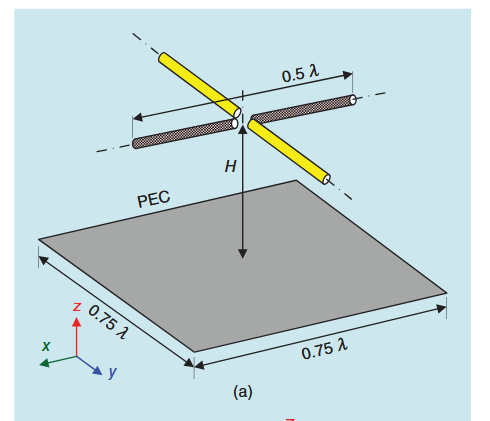
\includegraphics[width=0.5\linewidth]{crossed_dipole_antenna.png}
    \caption{A crossed dipole antenna \cite{7293591}}
    \label{fig:placeholder}
\end{figure}

A crossed dipole antenna radiates very evenly into every direction. This could be interesting to use, in order to excite several modes, especially in the presence of shielding materials.

When this antenna is near a perfect electric conductor (PEC), the gain becomes dependent on the distance to it. At a distance of $H=0.25\lambda$, the gain reaches a maximum due to constructive interference in normal direction to the PEC surface. When the distance is small, the image currents may cancel and the gain decreases. Therefore, the output power on the TEM cells depends on the distance, and implicitly on the frequency. This means that the frequency behavior of the representing dipoles may vary from a standard dipole.

Additionally, when a shielding material is present, different modes may be excited, which also influence the behavior. Those different modes depend on all 6 dipole moments, with which the antenna shall be modeled. 
